\documentclass{article}
\usepackage{arxiv}

\usepackage[utf8]{inputenc}
\usepackage[T2A]{fontenc}
\usepackage[english, russian]{babel}
\usepackage{url}
\usepackage{booktabs}
\usepackage{amsfonts}
\usepackage{amsthm}
\usepackage{amssymb}
\usepackage{amsmath}
\usepackage{nicefrac}
\usepackage{microtype}
\usepackage{graphicx}
\usepackage[square,sort,comma,numbers]{natbib}
\usepackage{doi}
\usepackage{algorithm}
\usepackage{algorithmic}


\newcommand{\argmin}{\arg\!\min}
\newcommand{\argmax}{\arg\!\max}


\title{Автоматическая регуляризация байесовских нейронных сетей}

\author{
    Басов Дмитрий Константинович
}
\date{}

\renewcommand{\shorttitle}{Автоматическая регуляризация байесовских нейронных сетей}
\numberwithin{equation}{section}

\begin{document}
    \maketitle

    \begin{abstract}
        В байесовском выводе, в отличие от гипотезы максимального правдоподобия,
        не делается никаких предположений о размере обучающей выборки.
        Это делает байесовские модели устойчивыми к переобучению.

        Однако применение байесовского подхода сопряжено с такими проблемами,
        как задание подходящего априорного распределения и вычисление апостериорного распределения весов модели.

        В данной работе предлагается следующее решение этих проблем:
        \begin{enumerate}
            \item Применяя вариационный вывод,
                мы аппроксимируем апостериорное распределение весов модели
                нормальным распределением с диагональной матрицей ковариации,
                и задача сводится к максимизации нижней вариационной границы.
                В этом случае каждый вес модели определяется двумя обучаемыми параметрами.
            \item Априорное распределение весов модели задается в виде
                нормального распределения с нулевым математическим ожиданием
                и диагональной матрицей ковариации, элементы которой вычисляются из данных.
                Этот приём лежит в основе Relevance Vector Machine (RVM)~--- байесовского варианта Support Vector Machine (SVM).
        \end{enumerate}

        Полученную модель можно рассматривать как
        ансамбль из бесконечного числа нейронных сетей,
        веса которых сэмплируются из нормального распределения.
        При этом каждый вес имеет свой индивидуальный коэффициент $L2$ регуляризации,
        который автоматически определяется из тренировочных данных при обучении.

    \end{abstract}

    \section{Обозначения и сокращения}
    $\pmb{x} \odot \pmb{y}$ --- поэлементное произведение (произведение Адамара) векторов \par
    $\mathcal{L}$ --- Evidence Lower Bound (ELBO) \par
    $
        KL(q~||~p)
        =
        \int_{}{
            q(\pmb{Z})
            \,
            \ln{
                \frac
                    {q(\pmb{Z})}
                    {p(\pmb{Z})}
            }
            \,
            d\pmb{Z}
        }
    $ --- дивергенция Кульбака--Лейблера (KL--дивергенции) \par
    $\pmb{x}$ --- вектор признаков \par
    $\pmb{y}$ --- вектор целевой переменной \par
    $D$ --- датасет --- пары значений $\{\pmb{x_i}$, $\pmb{y_i}\}$, где $i = 1, \dots, L$ \par
    $\pmb{W}$ --- веса модели --- случайная величина размерности M \par
    $p(\pmb{y} | \pmb{x}, D)$ --- предсказательное распределение \par
    $
        p(D | \pmb{W})
        =
        \prod_{i=1}^{L}{
            p(\pmb{y_i} | \pmb{x_i}, \pmb{W})
        }
    $ — правдоподобие (likelihood) \par
    $p(\pmb{W})$ --- априорное распределение весов модели (prior) \par
    $p(\pmb{W}| D)$ --- апостериорное распределение весов модели (posterior) \par
    $q_{\pmb{\theta}}(\pmb{W})$ --- аппроксимация апостериорного распределения весов модели \par
    $\pmb{\theta}$ --- обучаемые параметры байесовской модели \par

    \section{Введение}

    В классическом машинном обучении делается следующее предположение:
    веса модели $\pmb{W}$ являются пусть и неизвестной, но фиксированной величиной.
    В этом случае можно получить точечную оценку весов модели согласно гипотезе максимального правдоподобия:
    \begin{equation}\label{max_likelihood}
        \pmb{W_{ML}}
        =
        \argmax_{\pmb{W}} p(D | \pmb{W})
        =
        \argmax_{\pmb{W}} {
            \sum_{i=1}^{L}{
                \ln{
                    p(\pmb{y_{i}} | \pmb{x_{i}}, \pmb{W})
                }
            }
        }
    \end{equation}

    Тогда распределение $p(\pmb{y} | \pmb{x}, D)$ аппроксимируется следующим образом:
    \begin{equation}
        p(\pmb{y} | \pmb{x}, D) \approx p(\pmb{y} |\pmb{W_{ML}}, \pmb{x})
    \end{equation}

    Однако это справедливо при условии, что количество объектов в датасете D
    сильно больше количества весов модели ($L \gg M$).
    В противном случае веса модели $\pmb{W}$ могут слишком сильно подстроиться
    под обучающую выборку D, что может привести к переобучению.

    Для борьбы с переобучением используется ряд приёмов (штрафы на норму весов, early stopping, dropout),
    однако для их настройки требуются дополнительные вычислительные ресурсы
    и отложенные (не участвующие в обучении) выборки данных.

    Альтернативным подходом к машинному обучению является нахождение апостериорного распределения весов модели $p(\pmb{W}| D)$ по теореме Байеса:
    \begin{equation}
        p(\pmb{W}| D)
        =
        \frac
            {
                p(D | \pmb{W})
                \,
                p(\pmb{W})
            }
            {
                \int_{}{
                    p(D | \pmb{W})
                    \,
                    p(\pmb{W})
                    \,
                    d\pmb{W}
                }
            }
    \end{equation}

    Тогда предсказательное распределение $p(\pmb{y} | \pmb{x}, D)$ рассчитывается следующим образом:
    \begin{equation}
        p(\pmb{y} | \pmb{x}, D)
        =
        \int_{}{
            p(\pmb{y} | \pmb{x}, \pmb{W})
            \,
            p(\pmb{W} | D)
            \,
            d\pmb{W}
        }
    \end{equation}

    Байесовские модели можно рассматривать как ансамбль из бесконечного числа моделей,
    веса которых сэмплируются из распределения
    $p(\pmb{W}| D)$.
    Такой подход устойчив к переобучению, так как о размере обучающей выборки не делается никаких предположений.
    Однако возникают такие проблемы, как выбор подходящего априорного распределения
    $p(\pmb{W})$
    и вычисление апостериорного распределения
    $p(\pmb{W}| D)$.

    Неудачный выбор $p(\pmb{W})$ может сильно снизить качество модели,
    а расчёт апостериорного распределения $p(\pmb{W}| D)$
    требует вычисления интеграла по всему пространству весов модели,
    что для нейронных сетей практически невозможно.

    В данной статье предлагается следующий подход к решению этих проблем.

    \begin{enumerate}
        \item Применяя вариационный вывод,
            мы аппроксимируем распределение весов $p(\pmb{W}| D)$
            распределением $q_{\pmb{\theta}}(\pmb{W})$,
            и задача сводится к максимизации нижней вариационной границы
            $\mathcal{L}$ по параметрам $\pmb{\theta}$.
        \item Распределение $q_{\pmb{\theta}}(\pmb{W})$
            задаётся в виде нормального распределения с диагональной матрицей ковариации.
%             То есть каждый вес модели определяется двумя числами,
%             которые определяют его математическое ожидание и дисперсию.
%             Таким образом, количество обучаемых параметров
%             относительно классической нейронной сети возрастает в 2 раза.
        \item Так как распределение $q_{\pmb{\theta}}(\pmb{W})$
            является нормальным, применяя трюк с репараметризацией
            (reparameterization trick),
            становится возможным использовать градиентные методы
            для максимизации $\mathcal{L}$.
        \item Априорное распределение весов модели $p(\pmb{W})$
            задаётся в виде нормального распределения с нулевым математическим ожиданием
            и диагональной матрицей ковариации,
            элементы которой определяются при обучении из датасета D.
            Такой подход обладает большой универсальностью,
            однако из-за определения параметров априорного распределения $p(\pmb{W})$
            из данных D теряется теоретическая устойчивость к переобучению.
            Идея определения некоторых параметров априорного распределения
            $p(\pmb{W})$ из датасета D
            известна как эмпирический Байес.
        \item Вводятся новые параметры $\pmb{\gamma}$ и $\pmb{\rho}$,
            через которые выражаются математическое ожидание и дисперсия распределения
            $q_{\pmb{\theta}}(\pmb{W})$.
            Это позволяет избежать неопределенности деления $\dfrac{0}{0}$,
            которая может возникнуть из--за определения дисперсии распределения $p(\pmb{W})$ из данных.
    \end{enumerate}

    \section{Известные результаты}

    В \cite{mackay_1992a, mackay_1992b, mackay_1992c}
    рассматривается применение байесовского подхода к нейронным сетям,
    в том числе использование эмпирического Байеса
    для нахождения гиперпараметров.

    В работах \cite{mackay_1994, mackay_1995, nea_96}
    представлена техника Automatic Relevance Determination (ARD),
    которая легла в основу метода релевантых векторов (RVM) \cite{tipping_01},
    байесовского варианта метода опорных векторов (SVM).
    В отличие от SVM, RVM не требует подбора коэффициента регуляризации.

    В \cite{mackay_1992a, mackay_1992b, mackay_1992c, mackay_1994, mackay_1995}
    при вычислении апостериорного распределения весов модели использовалась
    аппроксимация Лапласа, а в \cite{nea_96} для сэмплирования весов
    из апостериорного распределения применялись методы
    Монте--Карло для марковских цепей (MCMC).
    Недостатком данных подходов являются сложности с масштабированием на большие модели.

    В работе \cite{hinton_van_camp_1993} была применена техника вариационного вывода
    для аппроксимации апостериорного распределения весов модели
    нормальным распределением с диагональной матрицей ковариации.
    Параметры распределения были найдены аналитически,
    что возможно только в случае нейронных сетей
    с одним скрытым слоем.

    В \cite{gra_11} для оценки параметров аппроксимации апостериорного распределения
    используются градиентные методы, что позволяет масштабировать вариационный вывод
    на большие модели.

    В \cite{blu_15} для обучения байесовской нейронной сети
    используется трюк с репараметризацией, который до этого был реализован в модели
    вариационного автокодировщика \cite{kingma_2013}.

    Различные способы задания априоных распределений весов
    байесовских нейронных сетей рассматриваются в
    \cite{nal_18, wi_20, hoe_21, for_22}.

    Обзор байесовских методов машинного обучения приведён в книгах
    \cite{bishop2006, murphy_book_1, murphy_book_2}.

    \section{Постановка задачи}

    Задача машинного обучения с учителем
    в вероятностной постановке формулируется следующим образом:
    необходимо получить распределение вероятностей
    $p(\pmb{y} | \pmb{x}, D)$
    целевой переменной $\pmb{y}$
    для неразмеченных $\pmb{x}$, используя информацию из датасета D.
    В случае параметрических моделей, которыми являются нейронные сети,
    информация из датасета D кодируется посредством весов модели $\pmb{W}$.
    Сделаем следующие преобразования:
    \begin{equation}\label{pred_distribution}
    \begin{split}
        p(\pmb{y} | \pmb{x}, D)
        =
        \int_{}{
            p(\pmb{y}, \pmb{W} | \pmb{x}, D)
            \,
            d\pmb{W}
        }
        =
        \int_{}{
            p(\pmb{y} | \pmb{W}, \pmb{x}, D)
            \,
            p(\pmb{W} | \pmb{x}, D)
            \,
            d\pmb{W}
        }
        =
        \int_{}{
            p(\pmb{y} | \pmb{W}, \pmb{x})
            \,
            p(\pmb{W} | D)
            \,
            d\pmb{W}
        }
    \end{split}
    \end{equation}

    Пояснения:
    \begin{itemize}
    \item
        $
            p(\pmb{y} | \pmb{x}, D)
            =
            \int_{}{
                p(\pmb{y}, \pmb{W} | \pmb{x}, D)
                \,
                d\pmb{W}
            }
        $, так как для любых случайных величин
        $\pmb{a}$ и $\pmb{b}$ справедливо
        $
            p(\pmb{a})
            =
            \int_{}{
                p(\pmb{a}, \pmb{b})
                \,
                d\pmb{b}
            }
        $;
    \item
        $
            p(\pmb{y}, \pmb{W} | \pmb{x}, D)
            =
            p(\pmb{y} | \pmb{W}, \pmb{x}, D)
            \,
            p(\pmb{W} | \pmb{x}, D)
        $, так как для любых случайных величин $\pmb{a}$ и $\pmb{b}$ справедливо
        $
            p(\pmb{a}, \pmb{b})
            =
            p(\pmb{a}| \pmb{b})
            \,
            p(\pmb{b})
        $;
    \item
        $
            p(\pmb{y} | \pmb{W}, \pmb{x}, D)
            =
            p(\pmb{y} | \pmb{W}, \pmb{x})
        $, так как вся информация из датасета D отражена в весах $\pmb{W}$;
    \item
        $
            p(\pmb{W} | \pmb{x}, D)
            =
            p(\pmb{W} | D)
        $, так как веса модели $\pmb{W}$ не зависят от неразмеченных
        $\pmb{x}$, которых не было в датасете D.
    \end{itemize}

    Таким образом, для получения предсказательного распределения $p(\pmb{y} | \pmb{x}, D)$
    необходимо получить распределение $p(\pmb{W}| D)$.
    Получим выражение для $p(\pmb{W}| D)$, используя формулу Байеса:
    \begin{equation}\label{posterior_distibution}
        p(\pmb{W}| D)
        =
        \frac
            {p(\pmb{W}, D)}
            {p(D)}
        =
        \frac
            {p(\pmb{W}, D)}
            {
                \int_{}{
                    p(\pmb{W}, D)
                    \,
                    d\pmb{W}
                }
            }
        =
        \frac
            {
                p(D | \pmb{W})
                \,
                p(\pmb{W})
            }
            {
                \int_{}{
                    p(D | \pmb{W})
                    \,
                    p(\pmb{W})
                    \,
                    d\pmb{W}
                }
            }
    \end{equation}

    Так как аналитическое вычисление интеграла в знаменателе (\ref{posterior_distibution})
    для нейронных сетей практически невозможно, возникает необходимость использовать различные аппроксимации
    для вычисления предсказательного распределения (\ref{pred_distribution}). Рассмотрим некоторые из них.

    \subsection{Точечная оценка весов модели}
    Вместо нахождения распределения весов $p(\pmb{W}| D)$
    можно сделать точечную оценку весов модели $\pmb{W}$.
    Эту оценку можно получить путём максимизации плотности вероятности весов $p(\pmb{W}| D)$:
    \begin{equation}\label{max_posterior}
        \pmb{W}^*
        =
        \argmax_{\pmb{W}}{
            p(\pmb{W} | D)
        }
        =
        \argmax_{\pmb{W}}{
            \ln{
                (
                    p(D | \pmb{W})
                    \cdot
                    p(\pmb{W})
                )
            }
        }
        =
        \argmax_{\pmb{W}} {
            (
                \sum_{i=1}^{L}{
                    \ln{
                        p(\pmb{y_{i}} | \pmb{x_{i}}, \pmb{W})
                    }
                }
                +
                \ln{p(\pmb{W})}
            )
        }
    \end{equation}

    $\pmb{W}^*$ называется максимальной апостериорной оценкой.
    Задание различных функциональных форм распределений
    $p(\pmb{y} | \pmb{x}, \pmb{W})$ и $p(\pmb{W})$
    эквивалентно различным функциям потерь, которые используются
    в классическом машинном обучении.
    Рассмотрим некоторые примеры:
    \begin{itemize}
        \item задание $p(\pmb{y} | \pmb{x}, \pmb{W})$ в виде распределения Бернулли
            равнозначно использованию логистической функции потерь;
        \item задание $p(\pmb{y} | \pmb{x}, \pmb{W})$ в виде нормального распределения
            равнозначно использованию метода наименьших квадратов;
        \item задание $p(\pmb{y} | \pmb{x}, \pmb{W})$ в виде распределения Лапласа
            равнозначно использованию метода наименьших модулей;
        \item задание $p(\pmb{W})$ в виде нормального распределения с нулевым математическим ожиданием
            равнозначно использованию L2 регуляризации,
            где коэффициент регуляризации определяется дисперсией априорного распределения;
        \item задание $p(\pmb{W})$ в виде распределения Лапласа с нулевым параметром сдвига
            равнозначно использованию L1 регуляризации,
            где коэффициент регуляризации определяется параметром масштаба априорного распределения;
        \item задание $p(\pmb{W})$ в виде равномерного распределения
            равнозначно отсутствию регуляризации,
            и максимальная апостериорная оценка (\ref{max_posterior}) превращается в
            оценку максимального правдоподобия (\ref{max_likelihood}).
    \end{itemize}

    Тогда предсказательное распределение (\ref{pred_distribution})
    аппроксимируется следующим образом:
    \begin{equation}
        p(\pmb{y} | \pmb{x}, D)
        =
        \int_{}{
            p(\pmb{y} | \pmb{W}, \pmb{x})
            \,
            p(\pmb{W} | D)
            \,
            d\pmb{W}
        }
        \approx
        p(\pmb{y} | \pmb{W}^*, \pmb{x})
    \end{equation}

    Обучаемыми параметрами являются веса модели $\pmb{W}^*$.
    Недостатом подхода точечной оценки весов модели является неустойчивость к переобучению.
    Для борьбы с переобучением используется множество приёмов,
    для настройки которых требуются дополнительные вычислительные ресурсы
    и валидационные (не участвующие в обучении) выборки данных.

    \subsection{MCMC}

    Для получения предсказательного распределения $p(\pmb{y} | \pmb{x}, D)$
    можно воспользоваться следующим подходом:
    используя методы Монте-Карло для марковских цепей (MCMC),
    из распределения $p(\pmb{W}| D)$ сэмплируются веса $\pmb{W}$.
    Тогда предсказательное распределение (\ref{pred_distribution})
    можно аппроксимировать следующим образом:
    \begin{equation}
        p(\pmb{y} | \pmb{x}, D)
        =
        \int_{}{
            p(\pmb{y} | \pmb{W}, \pmb{x})
            \,
            p(\pmb{W} | D)
            \,
            d\pmb{W}
        }
        \approx
            \frac{1}{T}
            \sum_{t=1}^{T}{
                p (
                    \pmb{y} | \pmb{x},
                    \pmb{\hat{W}_{t}}
                )
            }
    \end{equation}
    где $\pmb{\hat{W}_{t}}$~--- сэмпл весов модели из распределения $p(\pmb{W}| D)$
    и $T$~--- количество сэмплов для аппроксимации.
    Чем больше T, тем выше точность аппроксимации.

    Также стоит заметить, что в этом случае нет ни обучаемых параметров, ни функции потерь,
    которые присущи классическому машинному обучению.

    Однако сэмплирование весов из распределения $p(\pmb{W}| D)$ с использованием методов MCMC
    требует большого количества вычислительных ресурсов,
    что делает такой подход практически неприменимым для больших датасетов и большого числа весов.

    \subsection{Аппроксимация апостериорного распределения}

    Так как сэмплировать веса из распределения $p(\pmb{W}| D)$ вычислительно сложно,
    можно аппроксимировать апостериорное распределение $p(\pmb{W}| D)$
    распределением $q_{\pmb{\theta}}(\pmb{W})$, из которого сэмплировать намного проще.

    Тогда предсказательное распределение (\ref{pred_distribution})
    аппроксимируется следующим образом:
    \begin{equation}
        p(\pmb{y} | \pmb{x}, D)
        =
        \int_{}{
            p(\pmb{y} | \pmb{W}, \pmb{x})
            \,
            p(\pmb{W} | D)
            \,
            d\pmb{W}
        }
        \approx
        \int_{}{
            p(\pmb{y} | \pmb{W}, \pmb{x})
            \,
            q_{\pmb{\theta}}(\pmb{W})
            \,
            d\pmb{W}
        }
        \approx
            \frac{1}{T}
            \sum_{t=1}^{T}{
                p (
                    \pmb{y} | \pmb{x},
                    \pmb{\hat{W}_{t}}
                )
            }
    \end{equation}
    где $\pmb{\hat{W}_{t}}$~--- сэмпл весов модели из распределения $q_{\pmb{\theta}}(\pmb{W})$
    и $T$~--- количество сэмплов для аппроксимации.

    В этом случае обучаемыми параметрами являются $\pmb{\theta}$
    --- параметры распределения $q_{\pmb{\theta}}(\pmb{W})$,
    из которого сэмплируются веса $\pmb{W}$.
    Одним из подходов к аппроксимации сложного распределения более простым
    распределением является вариационный вывод.

    \section{Вариационный вывод}

    Идея вариационного вывода~--- сведение задачи байесовского вывода
    к задаче максимизации нижней вариационной границы (ELBO) $\mathcal{L}$,
    которая для распределения $q_{\pmb{\theta}}(\pmb{W})$
    записывается следующим образом:
    \begin{equation}
        \mathcal{L}
        =
            \int_{}{
                q_{\pmb{\theta}}(\pmb{W})
                \,
                \ln{
                    \frac
                        {p(\pmb{W}, D)}
                        {q_{\pmb{\theta}}(\pmb{W})}
                }
                \,
                d\pmb{W}
            }
    \end{equation}

    Покажем мотивацию максимизации $\mathcal{L}$.
    Запишем выражение для
    $
    KL(
        q_{\pmb{\theta}}(\pmb{W})
        \parallel
        p(\pmb{W}| D)
    )
    $
    и преобразуем его, используя тождество $p(\pmb{W}, D) = p(\pmb{W}| D) \, p(D)$:
    \begin{equation}
    \begin{split}
        KL(
            q_{\pmb{\theta}}(\pmb{W})
            \parallel
            p(\pmb{W}| D)
        ) = \\
        =
            \int_{}{
                q_{\pmb{\theta}}(\pmb{W})
                \,
                \ln{
                    \frac
                        {
                            q_{\pmb{\theta}}(\pmb{W})
                        }
                        {p(\pmb{W} | D)}
                }
                d\pmb{W}
            }
        = \\
        =
            \int_{}{
                q_{\pmb{\theta}}(\pmb{W})
                \,
                \ln{
                    \frac
                        {
                            p(D)
                            \,
                            q_{\pmb{\theta}}(\pmb{W})
                        }
                        {p(\pmb{W}, D)}
                }
                d\pmb{W}
            }
        = \\
        =
            \ln{p(D)}
            \,
            \int_{}{
                q_{\pmb{\theta}}(\pmb{W}) d\pmb{W}
            }
            -
            \int_{}{
                q_{\pmb{\theta}}(\pmb{W})
                \,
                \ln{
                    \frac
                        {p(\pmb{W}, D)}
                        {q_{\pmb{\theta}}(\pmb{W})}
                }
                d\pmb{W}
            }
        = \\
            \ln{p(D)} - \mathcal{L}
    \end{split}
    \end{equation}

    Так как $\ln{p(D)}$ не зависит от $\pmb{\theta}$,
    максимизация $\mathcal{L}$ по параметрам $\pmb{\theta}$
    ведёт к минимизации
    $KL(q_{\pmb{\theta}}(\pmb{W})~||~p(\pmb{W}| D))$.
    Таким образом, при максимизации $\mathcal{L}$
    распределение $q_{\pmb{\theta}}(\pmb{W})$
    будет приближаться к распределению $p(\pmb{W}| D)$.

    Преобразуем выражение для $\mathcal{L}$, используя тождество $p(\pmb{W}, D) = p(D | \pmb{W}) \, p(\pmb{W})$:
    \begin{equation}\label{elbo_inference}
    \begin{split}
        \mathcal{L}
        = \\
        =
            \int_{}{
                q_{\pmb{\theta}}(\pmb{W})
                \,
                \ln{
                    \frac
                        {p(\pmb{W}, D)}
                        {q_{\pmb{\theta}}(\pmb{W})}
                }
                d\pmb{W}
            }
        = \\
        =
            \int_{}{
                q_{\pmb{\theta}}(\pmb{W})
                \,
                \ln{
                    \frac
                        {
                            p(D | \pmb{W})
                            \,
                            p(\pmb{W})
                        }
                        {q_{\pmb{\theta}}(\pmb{W})}
                }
                d\pmb{W}
            }
        = \\
        =
            \int_{}{
                q_{\pmb{\theta}}(\pmb{W})
                \,
                \ln{
                    p(D | \pmb{W})
                }
                d\pmb{W}
            }
            -
            \int_{}{
                q_{\pmb{\theta}}(\pmb{W})
                \,
                \ln{
                    \frac
                        {q_{\pmb{\theta}}(\pmb{W})}
                        {p(\pmb{W})}
                }
                d\pmb{W}
            }
        = \\
        =
            \int_{}{
                q_{\pmb{\theta}}(\pmb{W})
                \,
                \ln{
                    p(D | \pmb{W})
                }
                d\pmb{W}
            }
            -
            KL(
                q_{\pmb{\theta}}(\pmb{W})~||~p(\pmb{W})
            )
    \end{split}
    \end{equation}

    Поставив
    $
        p(D | \pmb{W})
        =
        \prod_{i=1}^{L}{
            p(\pmb{y_i} | \pmb{x_i}, \pmb{W})
        }
    $
    в формулу (\ref{elbo_inference}), получим:
    \begin{equation}{\label{elbo_inference_ln}}
        \mathcal{L}
        =
            \int_{}{
                q_{\pmb{\theta}}(\pmb{W})
                \,
                \sum_{i=1}^{L}{
                    \ln{
                        p(\pmb{y_{i}} | \pmb{x_{i}}, \pmb{W})
                    }
                }
                d\pmb{W}
            }
            -
            KL(
                q_{\pmb{\theta}}(\pmb{W})~||~p(\pmb{W})
            )
    \end{equation}

    Таким образом, выражение для ELBO раскладывается на две составляющие.
    Левая часть показывает, насколько хорошо распределение весов модели
    $q_{\pmb{\theta}}(\pmb{W})$ описывает датасет D.
    Правая часть, которая является регуляризацией, показывает, насколько сильно распределение весов
    $q_{\pmb{\theta}}(\pmb{W})$ отличается от априорного распределения
    весов $p(\pmb{W})$.

    \section{Задание функциональных форм распределений}

    Для дальнейшнего вывода положим,
    что распределения $p(\pmb{W})$ и $q_{\pmb{\theta}}(\pmb{W})$
    являются нормальными с диагональными матрицами ковариации:
    \begin{equation}
        q_{\pmb{\theta}}(\pmb{W})
        =
            N(
                \pmb{W} | \pmb{\mu}, diag(\pmb{\sigma})^{2}
            )
        =
            \prod_{k=1}^M
            N(
                W_k | \mu_k, \sigma_k^2
            )
    \end{equation}

    \begin{equation}
        p(\pmb{W})
        =
            N(
                \pmb{W} | \pmb{0}, diag(\pmb{\delta})^{2}
            )
        =
            \prod_{k=1}^M
            N(
                W_k | 0, \delta_k^2
            )
    \end{equation}

    Так как распределения $p(\pmb{W})$ и $q_{\pmb{\theta}}(\pmb{W})$ нормальные, то
    $KL(q_{\pmb{\theta}}(\pmb{W})~||~p(\pmb{W}))$
    можно посчитать аналитически:
    \begin{equation}\label{kl_init}
        KL(
            q_{\pmb{\theta}}(\pmb{W})~||~p(\pmb{W})
        )
        =
            \frac{1}{2}\sum_{k=1}^{M}(
                \frac
                    {\sigma_{k}^2}
                    {\delta_{k}^2}
                +
                \frac
                    {\mu_{k}^2}
                    {\delta_{k}^2}
                -
                \ln{
                    \frac
                        {\sigma_{k}^2}
                        {\delta_{k}^2}
                }
                - 1
            )
    \end{equation}

    Подставив (\ref{kl_init}) в (\ref{elbo_inference_ln}), получим:
    \begin{equation}\label{elbo_kl}
        \mathcal{L}
        =
            \int_{}{
                q_{\pmb{\theta}}(\pmb{W})
                \,
                \sum_{i=1}^{L}{
                    \ln{
                        p(\pmb{y_{i}} | \pmb{x_{i}}, \pmb{W})
                    }
                }
                d\pmb{W}
            }
            -
            \frac{1}{2} \sum_{k=1}^{M}(
                \frac
                    {\sigma_{k}^2}
                    {\delta_{k}^2}
                +
                \frac
                    {\mu_{k}^2}
                    {\delta_{k}^2}
                -
                \ln{
                    \frac
                        {\sigma_{k}^2}
                        {\delta_{k}^2}
                }
                - 1
            )
    \end{equation}

    Таким образом,
    $\pmb{\mu}$ и $\pmb{\sigma}$~--- это обучаемые параметры модели,
    а параметр $\pmb{\delta}$~--- гиперпараметр
    (так как является параметром априорного распределения $p(\pmb{W})$).
    В байесовском выводе все параметры априорного распределения
    должны задаваться до начала обучения.
    Однако мы можем определить параметр $\pmb{\delta}$ из данных.
    Такой прием, как уже указывалось, называется эмпирический Байес.

    \section{Эмпирический Байес}
    Найдём такое значение $\pmb{\delta}$, при котором $\mathcal{L}$ максимальна.
    Так как в выражении (\ref{elbo_inference_ln})
    левое слагаемое не зависит от параметров распределения
    $p(\pmb{W})$, то максимум $\mathcal{L}$ достигается при минимуме
    $KL(q_{\pmb{\theta}}(\pmb{W})~||~p(\pmb{W}))$ по параметру $\pmb{\delta}$.

    Пусть $\pmb{\alpha} = diag(\pmb{\delta})^{-2}$.
    Тогда выражение (\ref{kl_init}) будет иметь следующий вид:
    \begin{equation}\label{kl_init_alpha}
        KL(
            q_{\pmb{\theta}}(\pmb{W})~||~p(\pmb{W})
        )
        =
            \frac{1}{2} \sum_{k=1}^{M} \left(
                \alpha_{k} \cdot \sigma_{k}^2
                + \alpha_{k} \cdot \mu_{k}^2
                - (\ln{\sigma_{k}^2} + \ln{\alpha_{k}})
                - 1
            \right)
    \end{equation}

    Найдём производную $KL(q_{\pmb{\theta}}(\pmb{W})~||~p(\pmb{W}))$ по параметру $\alpha_k$:
    \begin{equation}\label{kl_derivative}
        \frac
            {\partial (KL(q_{\pmb{\theta}}(\pmb{W})~||~p(\pmb{W})))}
            {\partial {\alpha_k}}
        =
            \frac{1}{2} \left(
                \sigma_{k}^2 + \mu_{k}^2 - \dfrac{1}{\alpha_k}
            \right)
        =
            \frac{1}{2} \left(
                \sigma_{k}^2 + \mu_{k}^2 - \delta_{k}^2
            \right)
    \end{equation}

    Приравняв (\ref{kl_derivative}) к нулю, получим выражение для оптимального значения $\pmb{\delta}$:
    \begin{equation}\label{delta_optim}
        \delta_{k}^2 = \sigma_{k}^2 + \mu_{k}^2
    \end{equation}

    Подставив (\ref{delta_optim}) в (\ref{elbo_kl}), получим:
    \begin{equation}\label{elbo_kl_optim}
        \mathcal{L}
        =
            \int_{}{
                q_{\pmb{\theta}}(\pmb{W})
                \,
                \sum_{i=1}^{L}{
                    \ln{
                        p(\pmb{y_{i}} | \pmb{x_{i}}, \pmb{W})
                    }
                }
                d\pmb{W}
            }
        -
            \frac{1}{2} \sum_{k=1}^{M} {
                \ln \left(
                    {1 + \frac{\mu_{k}^2}{\sigma_{k}^2}}
                \right)
            }
    \end{equation}

    Таким образом, задача свелась к максимизации $\mathcal{L}$
    по параметрам $\pmb{\mu}$ и $\pmb{\sigma}$.
    Покажем, как свести задачу максимизации $\mathcal{L}$ к задаче
    градиентной оптимизации.

    \section{Градиентная оптимизация}

    Так как в случае нейронной сети аналитически посчитать интеграл
    по всему пространству весов $\pmb{W}$ в (\ref{elbo_kl_optim}) не представляется возможным,
    воспользуемся следующей аппроксимацией для $\mathcal{L}$:
    \begin{equation}\label{elbo_kl_optim_sum}
        \mathcal{L}
        \approx
            \frac{1}{S} \sum_{j=1}^S \sum_{i=1}^{L} {
                \ln{
                    p(\pmb{y_{i}} | \pmb{x_{i}}, \pmb{\hat{W}_{ij}})
                }
            }
            -
            \frac{1}{2} \sum_{k=1}^{M} {
                \ln \left(
                    {1 + \frac{\mu_{k}^2}{\sigma_{k}^2}}
                \right)
            }
    \end{equation}

    где $\pmb{\hat{W}_{ij}}$~--- сэмпл весов модели из распределения
    $q_{\pmb{\theta}}(\pmb{W})$,
    $S$~--- количество сэмлов для аппроксимации,
    $L$~--- количество объектов в датасете D.

    Так как распределение $q_{\pmb{\theta}}(\pmb{W})$ нормальное,
    мы можем использовать трюк с репараметризацией при сэмплировании весов,
    что позволяет применять градиентные методы для оптимизации:
    \begin{equation}\label{w_trick}
        \pmb{\hat{W}_{ij}}
        =
            \pmb{\varepsilon_{ij}}
            \odot
            \pmb{\sigma}
            +
            \pmb{\mu}
    \end{equation}

    где $\pmb{\varepsilon_{ij}} \sim N(\pmb{0}, \pmb{I})$~--- сэмплы из стандартного
    нормального распределения.

    Задача максимизации (\ref{elbo_kl_optim_sum})
    свелась к градиентной оптимизации.
    Однако градиентная оптимизация $\mathcal{L}$ по параметрам $\pmb{\mu}$ и $\pmb{\sigma}$ может привести
    к численной нестабильности. Эта проблема решается заменой переменных.

    \section{Замена переменных}

    В некоторых случаях при максимизации $\mathcal{L}$
    какой-либо вес модели может перестать быть случайной величиной
    и выродиться в ноль
    ($\sigma_{k} \rightarrow 0$ и $\mu_{k} \rightarrow 0$).
    Это приведет к неопределенности деления 0 на 0
    при вычислении KL--дивергенции в (\ref{elbo_kl_optim_sum}).

    Также при градиентной оптимизации (\ref{elbo_kl_optim_sum})
    компоненты вектора $\pmb{\sigma}$ могут попасть в отрицательную область,
    что нежелательно, так как среднеквадратическое отклонение
    не может быть отрицательным по определению.

    Чтобы избежать этих проблем,
    определим параметры $\pmb{\sigma}$ и $\pmb{\mu}$
    через новые параметры $\pmb{\rho}$ и $\pmb{\gamma}$
    следующим образом:
    \begin{equation}\label{sigma_def}
        \pmb{\sigma}
        =
            \ln({
                1 + e^{\pmb{\rho}}
            })
        =
            Softplus (\pmb{\rho})
    \end{equation}

    \begin{equation}\label{mu_def}
        \pmb{\mu} = \pmb{\gamma} \odot \pmb{\sigma} = \pmb{\gamma} \odot Softplus (\pmb{\rho})
    \end{equation}

    Подставив (\ref{sigma_def}) и (\ref{mu_def}) в (\ref{elbo_kl_optim_sum}), получим:
    \begin{equation}\label{elbo_kl_optim_rho_gamma}
        \mathcal{L}
        \approx
            \frac{1}{S} \sum_{j=1}^S \sum_{i=1}^{L} {
                \ln{
                    p(\pmb{y_{i}} | \pmb{x_{i}}, \pmb{\hat{W}_{ij}})
                }
            }
        -
            \frac{1}{2} \sum_{k=1}^{M} \ln(
                {1 + \gamma_{k}^{2}}
            )
    \end{equation}

    Таким образом, задача свелась к максимизации (\ref{elbo_kl_optim_rho_gamma})
    по параметрам $\pmb{\rho}$ и $\pmb{\gamma}$.
    Значение $\pmb{\hat{W}_{ij}}$ вычисляется по (\ref{w_trick}),
    которое, в свою очередь, вычисляется через
    (\ref{sigma_def}) и (\ref{mu_def}).

    \section{Алгоритм обучения}
    Возьмем выражение для $\mathcal{L}$ из (\ref{elbo_kl_optim_rho_gamma}),
    и разделив на размер обучеющей выборки L со знаком минус,
    получим следующую функцию потерь:
    \begin{equation}\label{loss_init}
        loss(\pmb{\rho}, \pmb{\gamma})
        =
            - \frac
                {1}
                {S \cdot L}
            \sum_{j=1}^S
            \sum_{i=1}^{L}
                {\ln{
                    p(\pmb{y_{i}} | \pmb{x_{i}}, \pmb{\hat{W}_{ij}})
                }
            }
            +
            \frac
                {
                    \frac{1}{2} \sum_{k=1}^{M} \ln(
                        {1 + \gamma_{k}^{2}}
                    )
                }
                {L}
    \end{equation}

    Для ускорения расчёта функции потерь на каждом градиентном шаге введём следующие упрощения:
    \begin{itemize}
        \item на каждый объект будем делать только один сэмпл весов (то есть задать $S=1$);
        \item средний отрицательный логарифм правдоподобия будем считать не по всей обучающех выборке,
            а на случайном подмножестве (батче).
    \end{itemize}

    Тогда выражение (\ref{loss_init}) для функции потерь будет выглядить следующим образом:
    \begin{equation}\label{loss}
        loss(\pmb{\rho}, \pmb{\gamma})
        \approx
            - \frac{1}{B}
            \sum_{b=1}^{B}
                {\ln{
                    p(\pmb{y_{b}} | \pmb{x_{b}}, \pmb{\hat{W}_{b}})
                }
            }
            +
            \frac
                {
                    \frac{1}{2} \sum_{k=1}^{M} \ln(
                        {1 + \gamma_{k}^{2}}
                    )
                }
                {L}
    \end{equation}

    где:
    \begin{itemize}
        \item $\pmb{\rho}$ и $\pmb{\gamma}$~--- параметры распределения
            $q_{\pmb{\theta}}(\pmb{W})$ (обучаемые параметры модели);
        \item $\pmb{\hat{W}_{b}}$~--- сэмпл весов модели из распределения
            $q_{\pmb{\theta}}(\pmb{W})$;
        \item $B$~--- количество объектов в батче;
        \item $L$~--- количество объектов в датасете D;
        \item $M$~--- количество весов в модели.
    \end{itemize}

    Для минимизации (\ref{loss}) можно использовать любые методы градиентной оптимизации.
    Для наглядности рассмотрим алгоритм стохастического градиентного спуска.

    Задаем шаг градиентного спуска $\eta$ и инициализируем обучаемые параметры
    $\pmb{\rho}$ и $\pmb{\gamma}$.
    Затем повторяем, пока не достигнем критерия остановки:
    \begin{enumerate}
        \item
            $
                \pmb{\sigma}
                \leftarrow
                Softplus(\pmb{\rho})
            $ --- расчёт среднеквадратических отклонений весов
        \item
            $
                \pmb{\mu}
                \leftarrow
                    \pmb{\gamma}
                    \odot
                    \pmb{\sigma}
            $ --- расчёт математических ожиданий весов
        \item
            $
                \pmb{\varepsilon}
                \leftarrow
                N(0, 1)
            $ --- сэмплирование стандартного нормального шума
        \item
            $
                \hat{\pmb{W}}
                \leftarrow
                    \pmb{\varepsilon}
                    \odot
                    \pmb{\sigma}
                    +
                    \pmb{\mu}
            $ --- репараметризация
        \item
            $
                nll
                \leftarrow
                    -\dfrac{1}{B}
                    \sum_{b=1}^{B}{
                        \ln{
                            p(
                                \pmb{y_{b}} | \pmb{x_{b}}, \pmb{\hat{W}}
                            )
                        }
                    }
            $ --- расчёт среднего отрицательного логарифма правдоподобия
        \item
            $
                kl
                \leftarrow
                    \dfrac{1}{2}
                    \sum_{k=1}^{M}
                    \ln(
                        {1 + \gamma_{k}^{2}}
                    )
            $ --- расчёт KL--дивергенции
        \item
            $
                l
                \leftarrow
                    nll + \dfrac{kl}{L}
            $ --- расчёт функции потерь
        \item
            $
                \pmb{\rho}
                \leftarrow
                    \pmb{\rho}
                    -
                    \eta
                    \dfrac
                        {\partial l}
                        {\partial \pmb{\rho}}
            $ --- обновление $\pmb{\rho}$
        \item
            $
                \pmb{\gamma}
                \leftarrow
                    \pmb{\gamma}
                    -
                    \eta
                    \dfrac
                        {\partial l}
                        {\partial \pmb{\gamma}}
            $ --- обновление $\pmb{\gamma}$.
    \end{enumerate}

    \section{Эксперименты}
    Для проверки гипотезы был выбран
    \href
        {https://www.kaggle.com/datasets/rabieelkharoua/alzheimers-disease-dataset}
        {Alzheimer's Disease Dataset}.
    Данные были разбиты на тренировочную и тестовую часть в пропорции 80 на 20.
    В качестве архитектуры была выбрана полносвязная нейронная сеть с одним скрытым слоем и функцией активации ReLU, то есть: \\
    $z = ReLU(matmul(x, W_1))$ \\
    $y = Sigmoid(matmul(z, W_2))$.

    Размерность скрытого состояния $z$ варьировалась от 1 до 60.
    Для каждой размерности обучались 2 модели:
    классическая нейронная сеть и байесовская нейронная сеть.
    Для каждой модели производилась оценка ROC--AUC на тренировочной и тестовой выборках.

    Цель экспериментов: показать, что с увеличением сложности
    модели байесовская нейронная сеть не переобучается.

    \begin{figure}
        \centering
        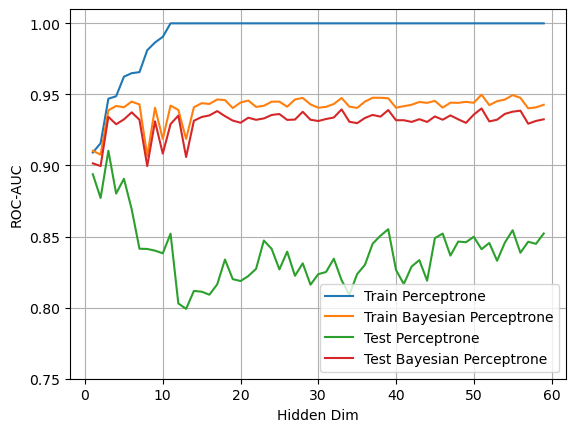
\includegraphics[width=1\linewidth]{roc_auc.png}
        \caption{Зависимость ROC--AUC от размерности скрытого состояния на тренировочных и тестовых данных}
        \label{graph_results}
    \end{figure}
    На рисунке \ref{graph_results} представлены результаты экспериментов.

    \section{Выводы}
    По результатам работы можно сделать следующие выводы:
    \begin{itemize}
        \item с ростом сложности модели байесовская нейронная сеть не переобучилась;
        \item значение ROC-AUC на тестовой выборке
        имеет очень высокую корреляцию со значением ROC-AUC на тренировочной выборке (0.97 по Пирсону).
        Следовательно, для подбора гиперпараметров можно ориентироваться на метрики,
        полученные на тренировочной выборке.
        Это даёт возможность отказаться от деления на тренировочную и валидационную выборки
        для подбора гиперпараметров.
    \end{itemize}

    Также стоит отметить,
    что данный подход переносится на другие архитектуры нейронных сетей
    (рекуррентные, свёрточные, трансформеры).

    Имплементация данного подхода была выполнена с использованием PyTorch.
    Весь исходный код для проведения экспериментов размещён по адресу
    \url{https://github.com/dimabasow/bayesian-neural-networks}.

\begin{thebibliography}{0}
    \bibitem{mackay_1992a}
        MacKay, D. J. C. (1992a).
        Bayesian interpolation. Neural Computation 4(3), 415–447.
    \bibitem{mackay_1992b}
        MacKay, D. J. C. (1992b).
        The evidence framework applied to classification networks.
        Neural Computation 4(5), 720–736.
    \bibitem{mackay_1992c}
        MacKay, D. J. C. (1992c).
        A practical Bayesian framework for back-propagation networks.
        Neural Computation 4(3), 448–472.
    \bibitem{mackay_1994}
        MacKay, D. J. C. (1994).
        Bayesian methods for backprop networks.
        In E. Domany, J. L. van Hemmen, and K. Schulten (Eds.),
        Models of Neural Networks, III, Chapter 6, pp. 211–254.
        Springer.
    \bibitem{mackay_1995}
        MacKay, D. J. C. (1995).
        Probable networks and plausible predictions~---
        a review of practical Bayesian methods for supervised neural networks”.
        In: Network: Computation in Neural Systems 6.3, pp. 469–505.
    \bibitem{nea_96}
        R. Neal. (1996).
        Bayesian learning for neural networks.
        Springer.
    \bibitem{tipping_01}
        Tipping, M. E. (2001).
        Sparse Bayesian learning and the relevance vector machine.
        Journal of Machine Learning Research 1, 211–244.
    \bibitem{hinton_van_camp_1993}
        Hinton, G. E. and D. van Camp (1993).
        Keeping neural networks simple by minimizing the description length of the weights.
        In Proceedings of the Sixth Annual Conference on Computational Learning Theory, pp. 5–13. ACM.
    \bibitem{gra_11}
        A. Graves (2011).
        Practical Variational Inference for Neural Networks.
        NIPS.
    \bibitem{blu_15}
        C. Blundell, J. Cornebise, K. Kavukcuoglu, and D. Wierstra. (2015).
        Weight Uncertainty in Neural Networks.
        ICML.
    \bibitem{kingma_2013}
        Kingma D. P., Welling M. (2013).
        Welling M. Auto-Encoding Variational Bayes. ArXiv e-prints.
    \bibitem{nal_18}
        E. T. Nalisnick. (2018).
        On Priors for Bayesian Neural Networks.
        PhD thesis. UC Irvine.
    \bibitem{wi_20}
        A. G. Wilson and P. Izmailov. (2020).
        Bayesian Deep Learning and a Probabilistic Perspective of Generalization.
        NIPS.
    \bibitem{hoe_21}
        T. Hoefler, D. Alistarh, T. Ben-Nun, N. Dryden, and A. Peste. (2021).
        Sparsity in Deep Learning:
        Pruning and growth for efficient inference and training in neural networks.
        In arXiv: 2102.00554.
    \bibitem{for_22}
        V. Fortuin. (2022).
        Priors in Bayesian Deep Learning: A Review.
        In: Intl. Statisical Review.
    \bibitem{bishop2006}
        C. Bishop (2006).
        Pattern recognition and machine learning.
        Springer.
    \bibitem{murphy_book_1}
        Kevin P. Murphy. (2022).
        Probabilistic Machine Learning: An introduction.
        MIT Press.
    \bibitem{murphy_book_2}
        Kevin P. Murphy. (2023).
        Probabilistic Machine Learning: Advanced Topics.
        MIT Press.
\end{thebibliography}


\end{document}
